% flashcards-title: Hundredths between one point two and one point three
% flashcards-desc: A number line from 1.20 to 1.30 has ten equal hundredth intervals and marks A at 1.26.
\documentclass[dvisvgm,tikz,border=8pt]{standalone}
\usetikzlibrary{arrows.meta,patterns}

\definecolor{qraNavy}{HTML}{17324D}
\definecolor{qraBlue}{HTML}{2B6CB0}
\definecolor{qraGold}{HTML}{B7791F}
\definecolor{qraPale}{HTML}{EAF2F8}
\definecolor{qraGray}{HTML}{5C6773}

\tikzset{
  qra axis/.style={draw=qraNavy, line width=1.2pt},
  qra tick/.style={draw=qraNavy, line width=1pt},
  qra guide/.style={draw=qraGray, densely dashed, line width=0.8pt},
  qra counter/.style={circle, draw=qraNavy, fill=qraPale, line width=0.9pt, minimum size=7mm, inner sep=0pt},
  qra label/.style={font=\sffamily\bfseries, text=qraNavy},
  qra small label/.style={font=\sffamily, text=qraNavy},
}

\begin{document}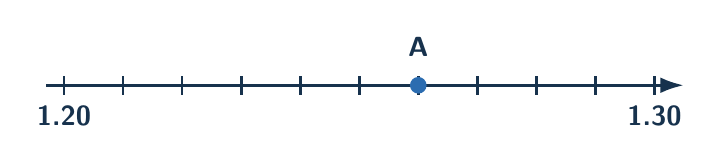
\begin{tikzpicture}[x=.75cm,y=1cm]
\draw[qra axis,-{Latex[length=3mm,width=2mm]}](-.3,0)--(10.5,0);\foreach \x in {0,...,10}{\draw[qra tick](\x,-.12)--(\x,.12);}
\node[qra label,below=4pt]at(0,0){1.20};\node[qra label,below=4pt]at(10,0){1.30};\fill[qraBlue](6,0)circle(3pt);\node[qra label,above=7pt]at(6,0){A};
\end{tikzpicture}\end{document}
